\documentclass[runningheads]{llncs}
\usepackage{hyperref}
\usepackage{amsmath}
\usepackage[T1]{fontenc}
\author{}
\institute{}
% T1 fonts will be used to generate the final print and online PDFs,
% so please use T1 fonts in your manuscript whenever possible.
% Other font encondings may result in incorrect characters.
%
\usepackage{graphicx}
% Used for displaying a sample figure. If possible, figure files should
% be included in EPS format.
%
% If you use the hyperref package, please uncomment the following two lines
% to display URLs in blue roman font according to Springer's eBook style:
%\usepackage{color}
%\renewcommand\UrlFont{\color{blue}\rmfamily}
%
\usepackage{arabtex}
\usepackage{utf8}
\begin{document}
%
\title{Bootless Application of Greedy Re-ranking Algorithms in Fair Neural Team Formation}

\titlerunning{Bootless Application of Greedy Re-ranking Algorithms ...}
% If the paper title is too long for the running head, you can set
% an abbreviated paper title here

\author{Hamed Loghmani\and
Hossein Fani\\\orcidID{\texttt{0000-0002-3857-4507}}^, \orcidID{\texttt{0000-0002-6033-6564}} }

\authorrunning{H. Loghmani and H. Fani.}
% First names are abbreviated in the running head.
% If there are more than two authors, 'et al.' is used.

\institute{University of Windsor, Canada\\ 
\email{\{ghasrlo, hfani\}@uwindsor.ca}}
%
\maketitle              % typeset the header of the contribution
%
\begin{abstract}
Team formation aims to automate forming teams of experts who can successfully solve difficult tasks, which have firsthand effects on creating organizational performance. While state-of-the-art neural team formation methods are able to efficiently analyze massive collections of experts to form effective collaborative teams, they largely ignore the fairness in recommended teams of experts. Fairness breeds innovation and increases teams' success by enabling a stronger sense of community, reducing conflict, and stimulating more creative thinking. In this paper, we study the application of state-of-the-art deterministic greedy re-ranking algorithms to mitigate the potential popularity bias in the neural team formation models based on \textit{equality of opportunity}. Our experiments show that, first, neural team formation models are biased toward popular experts. Second, although deterministic re-ranking algorithms mitigate popularity bias substantially, they severely hurt the efficacy of teams. The code to reproduce the experiments reported in this paper is available at \texttt{https://github.com/fani-lab/Adila/tree/bias23}\footnote{\setcode{utf8} A feminine Arabic given name, \<عادلة>, meaning just and fair.}.


% \keywords{Neural Team Formation  \and Popularity Bias \and Fairness.}
\end{abstract}
%
%
%
\section{Introduction}
% \vspace{-1em}
Algorithmic search for collaborative teams, also known as team formation, aims to automate forming teams of experts whose combined skills, applied in coordinated ways, can successfully solve complex tasks such as producing the next blockbuster \textit{`thriller'} with a touch of \textit{`sci-fi'} in the movie industry. Team formation can be seen as social information retrieval (Social IR) where the right group of talented people are searched and hired to solve the task at hand~\cite{10.1145/1772690.1772735,10.1145/2133806.2133830}. Successful teams have firsthand effects on creating organizational performance in the industry~\cite{156562,math8101804,Kairgalievna2021THEEO}, academia~\cite{YouEtAl99,doi:10.1146/annurev-soc-081715-074219,teamscience}, law~\cite{doi:10.1177/001979399504800405,Hu2014MakingAD}, and the healthcare sector~\cite{PMID:26182585,Rosen2018433}. Forming a successful team whose members can effectively collaborate and deliver the outcomes within the constraints such as planned budget and timeline is challenging due to the immense number of candidates with various backgrounds, personality traits, and skills, as well as unknown synergistic balance among them; not \textit{all} teams with the best experts are necessarily successful~\cite{doi:10.1177/0956797614537280}.

Historically, teams have been formed by relying on human experience and instinct, resulting in suboptimal team composition due to (1) an overwhelming number of candidates, and (2) hidden societal biases, among other reasons. To address the former, the earliest algorithmic methods of team formation were conceived in the \textit{i}) Operations Research (OR)~\cite{RAHMANNIYAY2019153}, where multiple objective functions must be optimized in a large search space of \textit{all} possible combinations of skillful experts, given constraints for human and non-human factors as well as scheduling preferences. Such work, however, was premised on the mutually independent selection of experts and overlooked the organizational and collaborative ties among experts. Next, \textit{ii}) social network analysis has been employed to fill the gap by the network representation of the experts with links that shows collaborations in the past \cite{DBLP:conf/kdd/LappasLT09,kargar2011discovering,6228185}.  They search for the optimum teams over \textit{all} possible subnetworks, which is daunting. Recently, \textit{iii}) a paradigm shift to machine learning has been observed, opening doors to the analysis of massive collections of experts coming from different fields. Machine learning approaches efficiently learn relationships between experts and their skills in the context of successful (positive samples) and unsuccessful teams (negative samples) from all past instances to excel at recommending teams of experts~\cite{DBLP:conf/cikm/RadMFKSB21,DBLP:conf/cikm/DashtiSF22,DBLP:conf/cikm/RadFKSB20}. We can observe the commercial application of machine learning-based algorithmic search for an optimum team in online platforms like LinkedIn\footnote{\href{https://business.linkedin.com/talent-solutions}{business.linkedin.com/talent-solutions}} to help the industry browse the enormous space of experts and form \textit{almost surely} successful teams.

However, the primary focus of existing machine learning-based methods in team formation is the maximization of the success rate (utility) by tailoring the recommended experts for a team to the required skills only, largely ignoring the \textit{fairness} in recommended experts. Indeed, it has been well-explored that machine learning methods that produce recommendations suffer from unfair biases. They result in discrimination and reduced visibility for an already disadvantaged group~\cite{DBLP:conf/innovations/DworkHPRZ12,DBLP:conf/kdd/HajianBC16}, disproportionate selection of popular candidates~\cite{DBLP:journals/ipm/YalcinB21,DBLP:conf/kdd/Zhu0ZC21,DBLP:conf/kdd/SunGZZRHGTYHC20}, and over/under-representation and racial/gender disparities~\cite{DBLP:conf/chi/KayMM15} since they are trained on real-world datasets that already inherit hidden societal biases. On the other hand, social science research provides compelling evidence about the synergistic effects of diversity on team performance~\cite{tannenbaum2019sex,lauring2019performance,hofstra2020diversity}; diversity breeds innovation and increases teams' success by enabling a stronger sense of community and support, reducing conflict, and stimulating more creative thinking. 

Surprisingly, there is little to no fairness-aware algorithmic method that mitigates societal biases in team formation algorithms except that of the recent work by Barnabò et al.~\cite{barnabo2019algorithms} that proves fair team formation is NP-complete; therefore, computationally prohibitive for practical use. Recent state-of-the-art neural team formation models have \textit{weakly} attributed their performance gain to mitigating popularity bias inherent in the underlying real-world training data~\cite{DBLP:conf/cikm/RadFKSB20,DBLP:conf/cikm/DashtiSF22}. Rad et al. ~\cite{DBLP:conf/cikm/RadFKSB20} employed uncertainty in learnable parameters by variational Bayesian neural model, and Dashti et al.~\cite{DBLP:conf/cikm/DashtiSF22} applied \textit{virtually} negative samples from popular experts during the neural model learning procedure. However, they overlook substantiating the attribution by evidence using fairness metrics. 
\begin{figure*}[t]
\centering
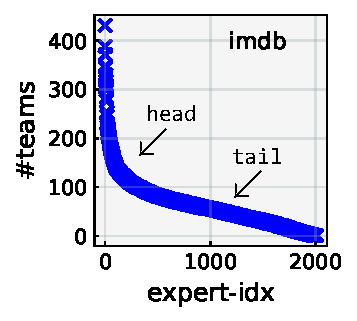
\includegraphics[scale=0.65]{figures/nteams_candidate-idx.pdf}
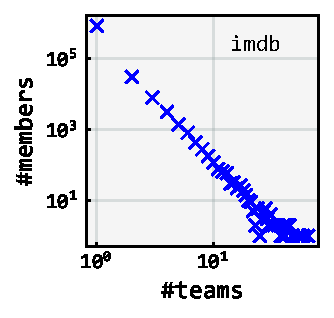
\includegraphics[scale=0.65]{figures/nmembers_nteams.pdf}
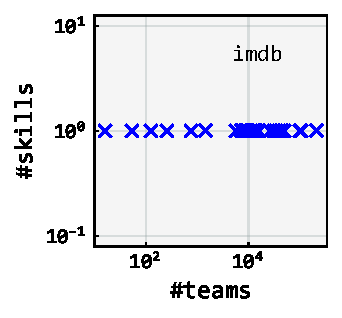
\includegraphics[scale=0.65]{figures/nskills_nteams.pdf}
\vspace{-1em}
\caption{Left: Long-tail distribution of casts and crews (experts) in movies (teams). Middle: Long-tail distribution in \texttt{log} scale. The figure reads $y$ number of members have $x$ number of teams. Right: uniform distribution of movies over genres (skills)} \label{fig:dist}
\vspace{-1em}
\end{figure*}

A purely diversity-centric design for team formation algorithms that solely overfit to satisfy diversity, neglecting the team's success, is also unfair to the organizations, e.g., a team of \textit{non}popular individuals who cannot accomplish the tasks. In this paper, we propose to model team formation as a two-sided marketplace between two stakeholders: \textit{i}) \textit{experts} who hold skills, e.g., artists, and \textit{ii}) \textit{organizations} who recruit experts for their teams, e.g., entertainment industries. We investigate the trade-off between success rate (utility) and fairness in the recommended teams by neural team formation methods in terms of popularity bias, given the required skills. The choice of popularity bias in this study is motivated due to: (1) training sets in team formation suffer from popularity bias; that is, the majority of experts have scarcely participated in the (successful) teams (nonpopular experts), whereas few experts (popular ones) are in many teams~\cite{DBLP:conf/cikm/RadFKSB20,DBLP:conf/cikm/DashtiSF22}. Therefore, popular experts receive higher scores and are more frequently recommended by the machine learning model, leading to systematic discrimination against already disadvantaged nonpopular experts. Statistically, popularity bias can be observed as long tail distribution (power law). For instance, in \texttt{imdb}\footnote{\href{https://imdb.com/interfaces/}{imdb.com/interfaces/}} dataset of movies, given a movie as a team of casts and crews such as actors and directors~\cite{DBLP:journals/tkde/KargarGSSZ22,kargar2011discovering}, from Fig.~\ref{fig:dist}(left), we observe a long tail of many nonpopular experts, while few popular experts in the head that dominate. Fig. ~\ref{fig:dist}(middle) shows the same observation in \texttt{log} scale based on $y$ number of experts participating in $x$ number of teams. (2) Moreover, experts' labels of being popular or otherwise can be calculated from datasets based on their position in the statistical distribution; that is, those in the \textit{`tail'} are assumed to be nonpopular experts, while those in the \textit{`head'} are the popular ones.  

In this paper, we employ the framework by Geyik et al.~\cite{DBLP:conf/kdd/GeyikAK19} for quantifying and mitigating popularity bias in state-of-the-art neural team formation methods~\cite{DBLP:conf/cikm/DashtiSF22} in terms of normalized discounted cumulative KL-divergence (\texttt{ndkl}) for \textit{re}ranking experts in the recommended teams to achieve fairness based on the \textit{equality of opportunity} (equalized odds)~\cite{hardt2016equality} depending on the distribution of teams over popular and nonpopular experts in the training datasets. Meanwhile, we measure the impact of the popularity bias mitigation on the success rate (utility) of the recommended teams using information retrieval metrics, namely mean average precision (\texttt{map}) and normalized discounted cumulative gain (\texttt{ndcg}). Our early results on \texttt{imdb} using three re-ranking algorithms by Geyik et al.~\cite{DBLP:conf/kdd/GeyikAK19} demonstrate that (1) state-of-the-art Bayesian neural models fall short in producing fair teams of experts in terms of popularity, and (2) state-of-the-art deterministic re-ranking algorithms improve the fairness of neural team formation models but at the cost of a substantial decrease in accuracy of predicted teams in terms of success rate. Our findings encourage further development of fairness-aware re-ranking methods for the task of team formation.

\section{Research Methodology}
% \vspace{-1em}
Ranking is the primary output interface of the neural team formation model for producing expert recommendations where all available experts are recommended for a given required subset of skills but with different scores, usually a probability value after a \texttt{softmax} layer, and the final recommended experts are selected among the top-$k$ highest scores. This enables further post-processing refinements like re-ranking the list of recommended items to improve fairness in the recommended list. Therefore, our research includes two pipelined steps: \textit{i}) training state-of-the-art neural team formation model to produce experts recommendations for given subsets of skills while measuring the accuracy and diversity of top-$k$ experts as the optimum team, and \textit{ii}) applying state-of-the-art re-ranking algorithms to reorder the top-$k$ experts and to improve fairness while maintaining accuracy. For example, when two or more experts have been assigned the same probability score in the final ranked list by a model, a re-ranking algorithm can prioritize nonpopular experts over popular ones and reassign new higher scores. 

We follow the \textit{equality of opportunity}~\cite{hardt2016equality} notion of fairness; that is, for being a member of a team (a preferred label that benefits an expert), a neural team formation model should predict an expert's membership with equal odds based on the underlying training dataset for all popular and nonpopular experts. In other words, equality of opportunity measures whether the experts who should qualify for a team are equally \textit{likely} regardless of their popularity status. For instance, given the percentage of popular experts to nonpopular ones is 10\% to 90\%, the neural model satisfies equality of opportunity for forming a team of $k$ experts should the team include $k\times 10\%$ popular and $k\times 90\%$ nonpopular experts. It is noteworthy that a \texttt{random} baseline that assigns experts to teams from a uniform distribution of experts regardless of popularity labels is an \textit{ideally} fair model yet at the cost of very low success rates for the predicted teams.

Intuitively, a few popular experts who participated in  many training instances of teams reinforce a neural model to forget about the majority nonpopular experts for their scarce number of teams, leading to popularity bias. As a result, a new predicted team would only include experts from the minority popular experts ($k\times 100\%$), which is disproportionate compared to their population size (10\%). In this paper, we aim to dampen the popularity bias by adjusting the distributions of popular and nonpopluar experts in the top-$k$ recommended experts for a team according to their ratio in the training dataset via deterministic algorithms and study the impacts on the team's quality in terms of success rate; that is measuring the accuracy of top-$k$ experts for teams whose all $k\times 100\%$ members are popular experts compared to teams with $k\times 10\%$ popular and $k\times 90\%$ nonpopular experts. 

% In the following, we formalize our research pipeline.

% \subsection{Neural Team Formation}
% Neural team formation finds an \textit{optimal} team of experts who collectively hold a set of required skills to yield success. Given a set of skills $\mathcal{S}$ and a set of experts $\mathcal{E}$, $(s, e)$ is a team of experts $e \subseteq \mathcal{E}$, that collectively hold a subset of skills $s \subseteq \mathcal{S}$, and $\mathcal{T} = \{((s, e), y); y \in \{0, 1\}\}$ indexes all successful and unsuccessful teams. A neural model estimate a mapping function $f$ of parameters $\theta$ from a subset of skills $s$ and experts $e$ to a boolean set; $f_{\theta}: \mathcal{P}(\mathcal{S}) \times \mathcal{P}(\mathcal{E}) \rightarrow \{0, 1\}$ given all previous collaborations $\mathcal{T}$ while maximizing the average log probability of teams' success or failure:
% \begin{equation}
%  \frac{1}{|\mathcal{T}|} \sum_{((s, e), y) \in \mathcal{T}} \log \text{P}(y|(s, e)) \label{eq:1}
% \end{equation}
% where $(s, e)$ is a team of experts $e$ who collectively hold the set of skills $s$ and can either work successfully together or fail otherwise. State-of-the-art neural models learn vector representations for experts and skills in the same vector space such that vectors of experts whose teams have been successful for the required skills will end up closer to each other while vectors of experts whose teams for the required skills have been unsuccessful will end up distant. They estimate $\text{P}(y|(s, e))$ through pairwise cosine similarities of vector representations for the skills and experts. Specifically, for a successful team $((s, e) , y = 1)$, $\text{P}(y = 1|(s, e))$ is estimated by learning $v_s=\sum_{i\in s}{v_i}$ and $v_e=\sum_{j\in e}{v_j}$ that are close in the vector space and have high cosine similarity while for an unsuccessful team $((s, e), y = 0)$, $\text{P}(y = 0|(s,  e))$ is estimated by learning $v_s$ and $v_e$ that are far from each other and have low cosine similarity. Formally, $\text{P}(y|(s, e))$ can be formulated using the \texttt{sigmoid} function $\sigma$:
% \begin{equation}
%  \text{P}(y|(s, e)) = \sigma(v^{\top}_{e} \cdot v_{s}) \label{eq:2}
% \end{equation}
% where $v_s$ and $v_e$ are the vector representations of the skill and expert subsets, respectively. 

% \subsection{Deterministic Reranking Methods}

\section{Experiments}
In this section, we lay out the details of our experiments and findings toward answering the following research questions:

\noindent\textbf{RQ1}: Do state-of-the-art neural team formation models produce fair teams of experts in terms of popularity bias? To this end, we benchmark state-of-the-art Bayesian neural model with negative sampling heuristics~\cite{DBLP:conf/cikm/DashtiSF22} and measure the fairness scores of predicted teams. 

\noindent\textbf{RQ2}: Do state-of-the-art deterministic greedy re-ranking algorithms improve the fairness of neural team formation models while maintaining their accuracy? To this end, we apply three deterministic greedy re-ranking algorithms on the neural model predictions and measure the diversity and utility scores afterwards.

\subsection{Setup}
% \vspace{-1em}
\subsubsection{Dataset.}
Our testbed includes \texttt{imdb}\cite{DBLP:journals/tkde/KargarGSSZ22,kargar2011discovering} dataset where each instance is a movie consisting of its cast and crew such as actors and director, as well as the movie's genres. We consider each movie as a team whose members are the cast and crew, and the movie's genres are the skills. The choice of \texttt{imdb} in team formation literature is not to be confused with its use cases in recommender systems or review analysis research; herein, the goal is to form a team of casts and crews for a movie production as opposed to a movie recommendation. As shown in Fig.~\ref{fig:dist}, we can observe a long tail in the distributions of teams over experts; many casts and crews have participated in very few movies. However, the distribution with respect to the set of skills follows a more fair distribution. Specifically, \texttt{imdb} has a limited variety of skills (genres) which are, by and large, employed by many movies. We filter out singleton and sparse movies with less than \texttt{3} members as well as casts and crews who relatively participated in very few movies, as suggested by~\cite{10.1145/3511808.3557590,DBLP:conf/cikm/RadFKSB20}. The latter also reduced the computational complexity of the neural models in their last layer where the size equals the number of experts. We ensured that the preprocessing step made no major change to the statistical distributions of the dataset. Table~\ref{tbl:stats} reports additional point-wise statistics on the dataset before and after preprocessing.
\subsubsection{Popularity Labels.} We label an expert as popular if she participated in more than the average number of teams per expert over the whole dataset, and nonpopular otherwise. As seen in Table~\ref{tbl:stats}, this number is \texttt{62.45} and the popularity ratio (popular/nonpopular) is \texttt{0.426/0.574}. 
\begin{table}[t]
% \scriptsize
\caption{Statistics of the raw and preprocessed \texttt{imdb} dataset.}
\label{tbl:stats}
\centering
\vspace{-1em}
\begin{tabular}{lcc}
\cline{2-3}
 & \multicolumn{2}{c}{\texttt{imdb}} \\ \cline{2-3} 
\multicolumn{1}{c}{} & raw & filtered \\ \hline
\#movies & 507,034 & 32,059 \\
\#unique casts and crews & 876,981 & 2,011 \\
\#unique genres & 28 & 23 \\
average \#casts and crews per team & 1.88 & 3.98 \\
average \#genres per team & 1.54 & 1.76 \\
average \#movie per cast and crew & 1.09 & 62.45 \\
average \#genre per cast and crew & 1.59 & 10.85 \\
\#team w/ single cast and crew & 322,918 & 0 \\
\#team w/ single genre & 315,503 & 15,180 \\ \hline
\end{tabular}
\vspace{-1em}
\end{table}
\subsubsection{Baselines.}
Our neural team formation baselines include variational Bayesian neural network~\cite{DBLP:conf/cikm/RadFKSB20} with unigram negative sampling strategy in minibatches~\cite{DBLP:conf/cikm/DashtiSF22} (\texttt{bnn}) and Kullback-Leibler optimization. The model includes a single hidden layer of size \texttt{d=100}, \texttt{leaky relu} and \texttt{sigmoid} are the activation functions for the hidden and the output layers, respectively, and \texttt{Adam} is the optimizer. The input and output layers are sparse occurrence vector representations (one-hot encoded) of skills and experts of size $|\mathcal{S}|$ and $|\mathcal{E}|$, respectively. Moreover, we also used pre-trained dense vector representations for the input skill subsets (\texttt{-emb}). Adapted from paragraph vectors of Le and Mikolov \cite{10.5555/3044805.3045025}, we consider each team as a document and the skills as the document's words. We used the distributed memory model to generate the real-valued embeddings of the subset of skills with a dimension of \texttt{d=100}. We evaluate baselines with and without the application of re-ranking methods (\texttt{before}, \texttt{after}). To have a minimum level of comparison, we also add a model that randomly assigns experts to a team (\texttt{random}). The re-ranking methods include the \textit{i}) score maximizing greedy mitigation algorithm (\texttt{greedy}), \textit{ii}) greedy conservative mitigation algorithm (\texttt{conservative}), and \textit{iii}) the relaxed variant of greedy conservative algorithm (\texttt{relaxed})~\cite{DBLP:conf/kdd/GeyikAK19}.
\subsubsection{Evaluation Strategy and Metrics.}
To demonstrate prediction effectiveness, we randomly select \texttt{15\%} of teams for the test set and perform \texttt{5}-fold cross-validation on the remaining teams for model training and validation that results in one trained model per each fold. Let $(s, e)$ a team of experts $e$ for the required skills $s$ from the test set, we compare the top-$k$ ranked list of experts $e'$, predicted by the model of each fold for the input skills $s$, with the observed subset of experts $e$ and report the average performance of models on all folds in terms of utility metrics (the higher, the better) including mean average precision (\texttt{map}) and normalized discounted cumulative gain (\texttt{ndcg}) at top-\{\texttt{2,5,10}\}. Formally,

\begin{align}
\texttt{ap}(k):\frac{\sum_{i=1}^{k}\texttt{p}(i)\times \delta_{e}(i)}{|{e}\cap e'|}
\end{align}
where $\texttt{p}(k)=\frac{|e\cap e'|}{k}$ is the precision, i.e., how many of the $k$ predicted experts $e'$ are correctly identified from the test instance of the team $e$ and $\delta_{e}(i)$ returns \texttt{1} if the $i$-th predicted expert is in $e$. Finally, we report the mean of average precisions  (\texttt{map}) on all test instances of teams. For normalized discounted cumulative gain (\texttt{ndcg}), 

\begin{align}
 \texttt{dcg}(k)=\sum_{i=1}^{k}\frac{\texttt{rel}(i)}{\texttt{log} (i+1)} \label{eq:2}
\end{align}
where $\texttt{rel}(i)$ captures the degree of relevance for the predicted expert at position $i$. In our problem setting, however, all members of a test team are considered of the same importance. Therefore, $rel(i)=\texttt{1}$ if $i \in e$ and \texttt{0} otherwise, and e.q.(\ref{eq:2}) becomes:
\begin{align}
\texttt{dcg}(k)=\sum_{i=1}^{k}\frac{\delta_{e}(i)}{\texttt{log}(i+1)} 
\end{align}
This metric can be {\it normalized} relative to the ideal case when the top-$k$ predicted experts include members of the test team $e$ at the lowest possible ranks, i.e.,
\begin{align}
\texttt{ndcg}(k)=\frac{\sum_{i=1}^{k}\frac{\delta_{e}(i)}{\texttt{log}(i+1)}}{\sum_{i=1}^{|e|}\frac{1}{\texttt{log}(i+1)}}
\end{align}

To evaluate fairness, we used \texttt{ndkl} with no cutoff~\cite{DBLP:conf/kdd/GeyikAK19} (the lower, the better) with being 0 in the ideal fair cases. Formally, let $d_{e'}$ the distribution of popular and nonpopular experts in the predicted top-$k$ experts $e'$ (the proportions of popular and nonpopular experts) and $d_e$ the ideal fair distribution for a test instance of a team $(s, e)$, the Kullback–Leibler (\texttt{kl}) divergence of $d_{e'}$ from $d_{e}$ is:

\begin{equation}
\texttt{kl}(d_{e'}(k)||d_e(k)) = \sum_{i=1}^{k} d_{e'}(i) \;\texttt{log} \frac{d_{e'}(i)}{d_e(i)}
\end{equation}
This metric has a minimum value of \texttt{0} when both distributions are identical up to position $i$. A higher value indicates a greater divergence between the two distributions, and the metric is always non-negative. We report the \textit{normalized  discounted cumulative} KL-divergence $(\texttt{ndkl})$\cite{DBLP:conf/kdd/GeyikAK19}:

\begin{equation}
\texttt{ndkl}(d_{e'}) = \frac{\sum_{k=1}^{|e|} \frac{1}{\texttt{log}(k+1)} \; \texttt{kl}(d_{e'}(k)||d_e(k))}{\sum_{i=1}^{|e|}\frac{1}{\texttt{log}(i+1)}}    
\end{equation}


\begin{table}[t]
\centering
%\scriptsize
\caption{Average performance of \texttt{5}-fold on test set in terms of fairness (\texttt{ndkl}; the lower, the better) and utility metrics (\texttt{map} and \texttt{ndcg}, the higher, the better) }
\vspace{-1em}
\begin{tabular}{cccccccc}\cline{3-8} 
\multicolumn{8}{c}{\texttt{bnn}\cite{DBLP:conf/cikm/DashtiSF22,DBLP:conf/cikm/RadFKSB20}}                                                                                                                                                \\ \cline{3-8} 
       &                                  & \multicolumn{2}{c|}{\texttt{greedy}}                 & \multicolumn{2}{c|}{\texttt{conservative}}              & \multicolumn{2}{c}{\texttt{relaxed}} \\ \cline{2-8} 
       & \multicolumn{1}{|c|}{\texttt{before}}      & \texttt{after}       & \multicolumn{1}{c|}{\texttt{\(\Delta \)}}        & \texttt{after}     & \multicolumn{1}{c|}{\texttt{\(\Delta \)}}             & \texttt{after}       & \texttt{\(\Delta \)}             \\ \hline \hline
\texttt{ndcg2$\uparrow$}  & \multicolumn{1}{|c|}{0.695\%}     & 0.126\%     & \multicolumn{1}{c|}{-0.569\%} & 0.091\%   & \multicolumn{1}{c|}{-0.604\%}      & 0.146\%      & -0.550\%      \\
\texttt{ndcg5$\uparrow$}  & \multicolumn{1}{|c|}{0.767\%}     & 0.141\%     & \multicolumn{1}{c|}{-0.626\%} & 0.130\%   & \multicolumn{1}{c|}{-0.637\%}      & 0.130\%      & -0.637\%      \\
\texttt{ndcg10$\uparrow$} & \multicolumn{1}{|c|}{1.058\%}     & 0.247\%     & \multicolumn{1}{c|}{-0.811\%} & 0.232\%   & \multicolumn{1}{c|}{-0.826\%}      & 0.246\%      & -0.812\%      \\\hline
\texttt{map2$\uparrow$}   & \multicolumn{1}{|c|}{0.248\%}     & 0.060\%     & \multicolumn{1}{c|}{-0.188\%} & 0.041\%   & \multicolumn{1}{c|}{-0.207\%}      & 0.063\%      & -0.185\%      \\
\texttt{map5$\uparrow$}   & \multicolumn{1}{|c|}{0.381\%}     & 0.083\%     & \multicolumn{1}{c|}{-0.298\%} & 0.068\%   & \multicolumn{1}{c|}{-0.313\%}      & 0.079\%      & -0.302\%      \\
\texttt{map10$\uparrow$}  & \multicolumn{1}{|c|}{0.467\%}     & 0.115\%     & \multicolumn{1}{c|}{-0.352\%} & 0.101\%   & \multicolumn{1}{c|}{-0.366\%}      & 0.115\%      & -0.352\%      \\ \hline \hline
\texttt{ndlkl$\downarrow$}  & \multicolumn{1}{|c|}{0.2317} & 0.0276 & \multicolumn{1}{c|}{-0.2041} & 0.0276 & \multicolumn{1}{c|}{-0.2041} & 0.0273 & -0.2043 \\ \hline
\end{tabular}
%\end{table}
\hfill
%\begin{table}[t]
\centering
\begin{tabular}{cccccccc}\cline{3-8} 
\multicolumn{8}{c}{\texttt{bnn\_emb}\cite{DBLP:conf/cikm/RadFKSB20,DBLP:conf/cikm/DashtiSF22}}                                                                                                                            \\ \cline{3-8} 
       &                              & \multicolumn{2}{c|}{\texttt{greedy}}             & \multicolumn{2}{c|}{\texttt{conservative}}       & \multicolumn{2}{c}{\texttt{relaxed}} \\ \cline{2-8} 
       & \multicolumn{1}{|c|}{\texttt{before}}  & \texttt{after}   & \multicolumn{1}{c|}{\texttt{\(\Delta \)}}        & \texttt{after}   & \multicolumn{1}{c|}{\texttt{\(\Delta \)}}        & \texttt{after}        & \texttt{\(\Delta \)}            \\ \hline \hline
\texttt{ndcg2$\uparrow$}  & \multicolumn{1}{|c|}{0.921\%} & 0.087\% & \multicolumn{1}{c|}{-0.834\%} & 0.121\% & \multicolumn{1}{c|}{-0.799\%} & 0.087\%      & -0.834\%     \\
\texttt{ndcg5$\uparrow$}  & \multicolumn{1}{|c|}{0.927\%} & 0.117\% & \multicolumn{1}{c|}{-0.810\%} & 0.150\% & \multicolumn{1}{c|}{-0.777\%} & 0.117\%      & -0.810\%     \\
\texttt{ndcg10$\uparrow$} & \multicolumn{1}{|c|}{1.266\%} & 0.223\% & \multicolumn{1}{c|}{-1.043\%} & 0.241\% & \multicolumn{1}{c|}{-1.025\%} & 0.223\%      & -1.043\%     \\ \hline
\texttt{map2$\uparrow$}   & \multicolumn{1}{|c|}{0.327\%} & 0.034\% & \multicolumn{1}{c|}{-0.293\%} & 0.057\% & \multicolumn{1}{c|}{-0.270\%} & 0.034\%      & -0.293\%     \\
\texttt{map5$\uparrow$}   & \multicolumn{1}{|c|}{0.469\%} & 0.059\% & \multicolumn{1}{c|}{-0.410\%} & 0.084\% & \multicolumn{1}{c|}{-0.386\%} & 0.059\%      & -0.410\%     \\
\texttt{map10$\uparrow$}  & \multicolumn{1}{|c|}{0.573\%} & 0.093\% & \multicolumn{1}{c|}{-0.480\%} & 0.111\% & \multicolumn{1}{c|}{-0.461\%} & 0.093\%      & -0.480\%     \\ \hline \hline
\texttt{ndkl$\downarrow$}   & \multicolumn{1}{|c|}{0.2779}                       & 0.0244  & \multicolumn{1}{c|}{-0.2535}  & 0.0244  & \multicolumn{1}{c|}{-0.2535}  & 0.0241       & -0.2539      \\ \hline
\label{tbl:bnn}
\end{tabular}
%\end{table}
\hfill
%\begin{table}[t]
\centering
\begin{tabular}{cccccccc}\cline{3-8}
\multicolumn{8}{c}{\texttt{random}}                                                                                                                                  \\ \cline{3-8} 
       &                                  & \multicolumn{2}{c}{\texttt{greedy}}              & \multicolumn{2}{c}{\texttt{conservative}}        & \multicolumn{2}{c}{\texttt{relaxed}} \\ \cline{2-8} 
       & \multicolumn{1}{|c|}{\texttt{before}}      & \texttt{after}   & \multicolumn{1}{c|}{\texttt{\(\Delta \)}}        & \texttt{after}   & \multicolumn{1}{c|}{\texttt{\(\Delta \)}}        & \texttt{after}        & \texttt{\(\Delta \)}            \\ \hline \hline
\texttt{ndcg2$\uparrow$}  & \multicolumn{1}{|c|}{0.1711\%} & 0.136\% & \multicolumn{1}{c|}{-0.035\%} & 0.205\% & \multicolumn{1}{c|}{0.034\%}  & 0.205\%      & 0.034\%      \\
\texttt{ndcg5$\uparrow$}  & \multicolumn{1}{|c|}{0.1809\%} & 0.170\% & \multicolumn{1}{c|}{-0.011\%} & 0.190\% & \multicolumn{1}{c|}{0.009\%}  & 0.190\%      & 0.009\%      \\
\texttt{ndcg10$\uparrow$} & \multicolumn{1}{|c|}{0.3086\%} & 0.258\% & \multicolumn{1}{c|}{-0.051\%} & 0.283\% & \multicolumn{1}{c|}{-0.026\%} & 0.283\%      & -0.026\%     \\ \hline
\texttt{map2$\uparrow$}   & \multicolumn{1}{|c|}{0.0617\%} & 0.059\% & \multicolumn{1}{c|}{-0.003\%} & 0.089\% & \multicolumn{1}{c|}{0.028\%}  & 0.089\%      & 0.028\%      \\
\texttt{map5$\uparrow$}   & \multicolumn{1}{|c|}{0.0889\%}  & 0.095\% & \multicolumn{1}{c|}{0.006\%}  & 0.110\% & \multicolumn{1}{c|}{0.021\%}  & 0.110\%      & 0.021\%      \\
\texttt{map10$\uparrow$}  & \multicolumn{1}{|c|}{0.1244\%} & 0.121\% & \multicolumn{1}{c|}{-0.003\%} & 0.140\% & \multicolumn{1}{c|}{0.016\%}  & 0.140\%      & 0.016\%      \\ \hline \hline
\texttt{ndkl$\downarrow$}   & \multicolumn{1}{|c|}{0.0072}      & 0.0369  & \multicolumn{1}{c|}{0.0296}   & 0.0366  & \multicolumn{1}{c|}{0.0293}   & 0.0366       & 0.0294       \\ \hline
\end{tabular}
%\end{table}
\vspace{-2em}
\end{table}
\subsection{Results}
In response to \textbf{RQ1}, i.e., whether state-of-the-art neural team formation models produce fair teams of experts, from Table~\ref{tbl:bnn}, we observe that state-of-the-art Bayesian neural models with negative sampling (\texttt{bnn} and \texttt{bnn\_emb}) suffer from popularity bias having regard to their high \texttt{ndkl} compared to \texttt{random} baseline \texttt{before} applying deterministic re-ranking algorithms, thus answering \textbf{RQ2} negatively. Indeed, the \texttt{random} baseline which blindly assigns experts to teams is following the experts' popularity label distribution in the training dataset, and hence, yields the best fair model based on \textit{equality of opportunity} (equalized odds). However, \texttt{random} baseline has the lowest utility metric values while \texttt{bnn} and \texttt{bnn\_emb} achieve the highest. 

In response to \textbf{RQ2}, i.e., whether state-of-the-art deterministic re-ranking algorithms improve the fairness of neural team formation models while maintaining their accuracy, from Table~\ref{tbl:bnn}, although applying all re-ranking algorithms resulted in lower \texttt{ndkl} values by increasing the diversity of experts in the recommended teams, they substantially reduced the teams' accuracy at the same time for all neural models in terms of all utility metrics, proving the ineffectiveness of deterministic greedy re-ranking algorithms for the task of team formation. Among the re-ranking algorithms, \texttt{relaxed} is the best since it decreases the \texttt{ndkl} of neural models the most while the drop in the utility metrics is the lowest compared to the other two algorithms.

\section{Concluding Remarks}
We focused on the problem of fair team formation. We showed that state-of-the-art neural models, which can efficiently learn relationships between experts and their skills in the context of successful and unsuccessful teams from all past instances, suffer from popularity bias. To mitigate the popularity bias while maintaining the success rates of recommended teams, we applied three state-of-the-art deterministic re-ranking algorithms to reorder the final ranked list of experts against the popular experts in favour of nonpopular ones. We found that while deterministic re-ranking algorithms improve the fairness of neural team formation models, they fall short of maintaining accuracy. Our future research directions include \textit{i}) investigating other fairness factors like demographic attributes, including age, race, and gender; and \textit{ii}) developing machine learning-based models using Learning-to-Rank (L2R) techniques to mitigate popularity bias as opposed to deterministic greedy algorithms.


%
% ---- Bibliography ----
%
% BibTeX users should specify bibliography style 'splncs04'.
% References will then be sorted and formatted in the correct style.
%
% \bibliographystyle{splncs04}
\bibliographystyle{unsrt}
\bibliography{ref}
%

\end{document}
